\documentclass[a4, twocolumn, 12pt]{article}
\usepackage[utf8]{inputenc}
\usepackage[a4paper,
            left=0.75in,right=0.75in,top=1.2in,bottom=1.2in,%
            footskip=.25in]{geometry}
\setlength{\columnsep}{20pt}

\usepackage{float}
\usepackage{nccmath}
\usepackage{enumitem}
\usepackage{amsmath}

%Includes "References" in the table of contents
\usepackage[nottoc]{tocbibind}

\providecommand{\keywords}[1]{\textbf{\textit{Keywords - }} #1}

\title{FROG Analytics \\
\large  Project Repository: https://github.com/adrian-pace/FROG-analytics}
\author{
Baligand Louis\\
\texttt{louis.baligand@epfl.ch}
\and
Pace Adrian\\
\texttt{adrian.pace@epfl.ch}
\and
Håklev Stian\\
\texttt{stian.haklev@epfl.ch}
\and
Olsen Jennifer\\
\texttt{jennifer.olsen@epfl.ch}
\and
Dillenbourg Pierre\\
\texttt{pierre.dillenbourg@epfl.ch}}
\date{\today}

\usepackage{graphicx}

\begin{document}

\maketitle
   
\begin{abstract}
This report covers the semester Project of the two master students L. Baligand and A. Pace under the supervision of S. Haklev and J. Olsen in the CHILI lab at EPFL. The aim of the project is to develop a stand-alone application that, through FROG's editor,   provides metrics for each document created and visualizes them in real time. These metrics aim at describing the collaboration between the authors when they write in the document.
\end{abstract}

\keywords{Collaborative writing, FROG, online editors}

\section{Introduction}
Collaborative writing as the name suggests, aims at bringing people together to work as a cohesive unit on a particular project. Traditional education systems and methods of teaching generally involve teachers assigning tasks to students who work on said task individually. However, criticism throughout the ages has shed light onto the fact that this formal method of imbibing knowledge has stripped the education system of any social dimension \cite{Bornstein}. Thus, collaborative writing strategies as a result of group interaction and through the means of strengthening individual cognitive skills, achieve this lacking dimension. 
\\
In this new age of technology, individuals now have access to social software and online platforms such as GoogleDoc, Etherpad and Wiki-that offer numerous distinctive and powerful information sharing and collaboration features such as allowing learners to actively participate in knowledge construction \cite{boulos}, improving co-writing processes and simplifying monitoring methods. 
 \\
 \\
Our work is based on the École Polytechnique Fédérale de Lausanne’s (EPFL) FROG program. FROG (Fabricate and Run Orchestration Graphs) is an open-source web-platform that supervises collaborative learning activities. It is accessed by professors to build and run pedagogical scripts \cite{haklev}.\\
The platform offers an array of activities, which include: topical videos, text reading analysis, collaborative report writing and even contributing ideas collectively. Hence providing abundant data that must be processed and utilised. This underlying fact is the key motivation for our strive to search and enhance the area of collaborative report writing.
\\
The aim of this project is to showcase analytics in real time to a teacher. This starts with building an entire server-based system, to compute algorithms and metrics that describe and contextualize what students are writing.

\section{Data}
The main goal of this project is to compute collaborative metrics from documents written on the FROG platform. However, in order to develop the system, it is easier to begin with simpler collaborative systems such as Etherpad and Collab-react-components. Following this, we test and optimize our system using information collected from two data sets that was written on the Etherpad editor. The two datasets are based on experiments run by Stian Håklev (will later be referred to as Stian’s logs) and a group of Belgian scientists (referred to as the Belgian experiment).
\\
Etherpad is a highly customizable open source online editor that provides collaborative editing in real-time. It allows multiple users to edit the same text document by writing on a webpage. One can add, delete or format text. It stores each writing event in a database. These writing events contain what the authors have done on the document. They are sampled every few milliseconds. In our report, we focus only on the additions and deletions. Each event is defined by its author, a timestamp at when it occurred, the document version (incremented at each writing event) and the changeset containing the modification. The changeset contains the position in the document at which the event takes place-what characters to delete and to add. These writing events can be written and stored in multiple database formats. While we focus on the SQLite3 and the dirty database format, many others are available. The SQLite3 format creates a file containing a SQLite3 database that contains the writing events. The dirty database format creates a file with all writing events.\\
Collab-react-components is a database backend and collaborative React editor. This was designed and developed by Dario Anongba as a part of his semester project for the CHILI lab; it is the system behind FROG’s editors. It works in a relatively similar manner as Etherpad, saving its writing events in a mongo database instead. \\
Stian’s logs is a collection of writing events on hundreds of documents written in Etherpad. The authors of each document were supposed to answer a sequence of questions collaboratively. This extensive amount of writing allows us to test our implementations in greater detail as the writing events from these numerous documents cover nearly every anomaly we can encounter. \\
The Belgian experiment is an experiment run by a team of Belgian scientists, where students were asked to write collaboratively on the documents, in a similar manner to Stian’s logs. The writing events are written in SQLite3 databases in Etherpad format. This experience is however better controlled and time-limited which yields more consistent documents in terms of quality and amount of writing in comparison to Stian’s logs. Since the authors of these documents were asked to fill a questionnaire about their collaborative writing skills, we use it to study whether their assessments are related to the way they write.
\\\\
Before investigating how we use these various datasets, let us first go through the details of the implementation to improve our understanding of how we represent the documents and how we compute our metrics.

\section{Architecture}
The system we build is a stand-alone application from FROG written in Python that communicates with the FROG server written in JavaScript through HTTP/POST requests. We will go through the execution of the program sequentially to have a better grasp of how the system extracts high level metrics from writing events.\\
We first start the program by starting the web server. It is based on a Flask framework as we expect its load to be relatively low as it only receives a few POST requests from FROG occasionally. These POST requests are what actually start the analytics. If the request does not contain a JSON payload, then the web server starts the analytics on all the documents that exist in the FROG Mongo database. If a JSON payload is present, it either explicitly specifies the documents we want to run the analytics on, or specifies the RegEx expression that the documents we run analytics on should match.\\
Upon the reception of a POST request, the web server starts two threads. This includes one update thread which sends at certain intervals, with the metrics for all the documents we are interested in to FROG in a POST request. The analytic thread is the bulk of our implementation. It first parses the database to create \texttt{ElementaryOperations}. It then groups the \texttt{ElemntaryOperations} into \texttt{Operations}. Following which, it then deduces the \texttt{Paragraphs} from a document. It classifies them into operation types and builds their context. Finally it computes the metrics for each document. Before we dig into the details of each step, it is important to note that this procedure needs to be run at regular intervals as the users continue writing on the editors after we have computed our metrics. As we will go into further detail, the parsing is able to parse only the new writing events it has never seen before. With the same logic, one will see that most of the stages are capable of processing these new writing events without rerunning the analysis on all the writing events.\\
We will study each stage individually and will define these new objects we have just mentioned. An example of the topology is shown on Fig.\ref{archi}.
\begin{figure}
\centering
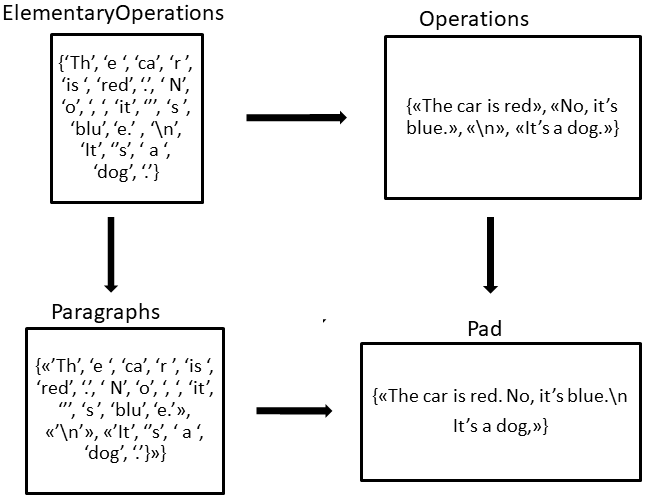
\includegraphics[scale=0.47]{figures/Archi.png}
\caption{Overview of the architecture}
\label{archi}
\end{figure}

\subsection{\texttt{ElementaryOperations} and Parsing}
The parsing can handle multiple databases. For a Mongo database (in the case of FROG’s or collab-react-components’ documents), we first connect to the database. If this is the first time we run the parsing, the system will fetch all the writing events from the database whose documents match the RegEx expression or the list of document names passed in the JSON of the POST request and creates one or multiple \texttt{ElementaryOperation} for each of these writing events. An \texttt{ElementaryOperation} is a python object that represents a writing event. It is mostly defined by its position, its type (add or del), its text to add or length to delete, its timestamp and its author. Sometimes the parser splits a writing event into two \texttt{ElementaryOperation}. This is usually the case when the writing events consist of changing a character for another (deletion followed by an addition). In these cases, we divide the event into a deletion and an addition. Since we need the deletion to be done before the addition, we increment the timestamp of the addition by 1 ms. We then add this offset to the following parsed \texttt{ElementaryOperations}. The next time, we parse the database, we only look for new writing events. Note that in each writing event, there is the document version number. Thus, in order to filter the writing events to parse only the new ones, we parse the database and keep track of the last version of each document. We can then query the database for all the writing events whose document version is higher than the last version we parsed for this document. We also query for documents we have never seen but match the RegEx expression or the list of document names passed in the JSON of the POST request. \\
For an Etherpad Database, we proceed in a similar manner. In the dirty DB (the database we first start working with), the writing events are written sequentially. We parse each event into one or multiple \texttt{ElementaryOperations}. The format of the writing event is different but the idea is the same as before. The next time we parse the database, we only fetch the new writing events. Instead of looking at the document version number, we now only keep track of the last line number we treated and handle all writing events that are after this line number, as writing events are written sequentially.\\
This is the general idea of how parsing is done on editors. Clearly there is some room for improvement in Etherpad. We could for example parse different database style and fetch the new writing events in the same way as the Mongo database-instead of fetching all the lines from the dirty DB and selecting only the last lines. We decide however not to focus on this enhancement since our main objective is to integrate our system with FROG.\\
We also have a special parsing function that can parse the dataset we are given-such as the Belgian experiment or Stian’s logs. These parsers are however not used by the analytics thread as the thread is designed to run on writing events databases that change in real-time. Although they are used in our testing analysis and parameter tuning study that we will discuss later on. Both Stian’s logs and the Belgian experiment are done in Etherpad. One was stored in a CSV file and the other in multiple SQLite3 databases (one database per document). The parsing of the databases is somewhat different but the transformation of each writing event into a \texttt{ElementaryOperation} is relatively similar to the previous Etherpad dirty database parser.

\subsection{\texttt{ElementaryOperations} and \texttt{Operations} Grouping}
Each \texttt{ElementaryOperation} usually contains between 1 to 3 characters depending on the writing speed of the user so it is difficult to gain any insight directly from the \texttt{ElementaryOperations} as they are so fine-grained. To solve this problem we group the \texttt{ElementaryOperation} into \texttt{Operations}. An Operation is mostly defined by its start position, its length, starting and ending timestamp, author and the list of \texttt{ElementaryOperation} it is composed of. It represents a thought-process. For example, if a user is writing a block of text without pausing for too long, the corresponding \texttt{ElementaryOperations} will be grouped into one \texttt{Operation}. If while writing the user decides to change a few characters in his block of text, the corresponding \texttt{ElementaryOperations} will still be in the same \texttt{Operation}. However if the user starts writing somewhere else in the document (not the block of text he first wrote in) then the corresponding \texttt{ElementaryOperations} will not be in the same \texttt{Operation} but will instead be part a newly created \texttt{Operation}.\\
A \texttt{Pad} simply represents the document. It is defined by the list of the \texttt{Operations} corresponding to this document and a pad name (the document name).\\
The way these \texttt{Operations} and \texttt{Pads} are built is by iterating over each new \texttt{ElementaryOperation} that the parser yields. For each \texttt{ElementaryOperation}, we check whether its document has a \texttt{Pad}. If so, we check whether its author had already been writing before. If yes, we then check whether the criterias are met for the \texttt{ElementaryOperation} to belong to the last \texttt{Operation} of the author. If this is the case, we add it to the \texttt{Operation} and update various attributes of the \texttt{Operation} such as its length, position, etc… If the criterias are not met, we add the last \texttt{Operation} of the author to the pad and create a new \texttt{Operation} containing our \texttt{ElementaryOperation}. This becomes the last \texttt{Operation} of the author (that might be completed with the next \texttt{ElementaryOperations}). If there is no last \texttt{Operation} for this author (this is the first time the author is writing), we simply create a new Operation. Finally if this is the first \texttt{ElementaryOperation} of the documents, we simply create a new \texttt{Pad}.\\
Once every \texttt{ElementaryOperation} has been processed, we yield back the \texttt{Pads}.\\
The next time we will run this procedure with the new \texttt{ElementaryOperations} yielded by the parser, we will also send to the method the existing Pads and the last \texttt{Operation} of each author. This way, it can add some of the new \texttt{ElementaryOperations} to an \texttt{Operation} that was started from the previous parsing.\\
A final remark is the extra computation that occurs if there is a new line in an \texttt{ElementaryOperation}. In the next processing steps, we need to keep track of the line number of each \texttt{ElementaryOperation}. Hence, if an \texttt{ElementaryOperation} contains a newline, it belongs to two lines which is not compatible with our processing. Therefore, we split this kind of \texttt{ElementaryOperation} along their new lines into multiple \texttt{ElementaryOperations}. The timestamp is also changed to differentiate these new multiple \texttt{ElementaryOperations} in a similar fashion as in the parsing. This way, an \texttt{ElementaryOperation} of type add either add only a newline or add text without newlines.\\
A visualization where all the \texttt{Operations} from a text are colored in a different random color each is shown on Fig. \ref{operations}
\begin{figure}
\centering
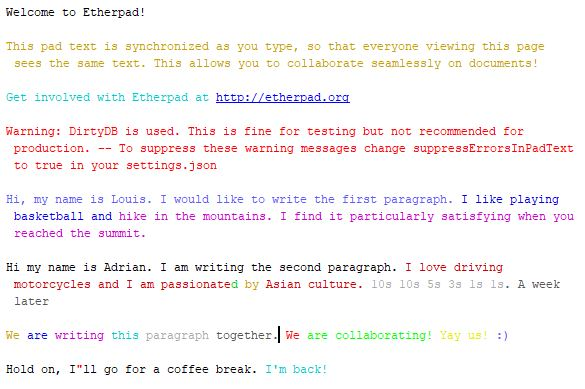
\includegraphics[scale=0.5]{figures/operations.JPG}
\caption{Display of a text with randomly colored \texttt{Operations}}
\label{operations}
\end{figure}



\subsection{\texttt{Paragraph}}
A \texttt{Paragraph} is the grouping of \texttt{ElementaryOperation} that are positioned in the same line. As we will later see, this is necessary for the \texttt{Operation} context calculation and the metrics computation. To create the paragraphs, the program iterates over all the new \texttt{ElementaryOperations} once they have been classified into \texttt{Operations} from the previous step. \\
If the \texttt{ElementaryOperation} is not a new line and affects only one paragraph, we add it to the paragraph it belongs to.
If it is an add \texttt{ElementaryOperation} adding a new line, we either create a new \texttt{Paragraph}, or split the \texttt{Paragraph} it is in the middle of along the position of the \texttt{ElementaryOperation}. In the latter case, the \texttt{ElementaryOperations} belonging to the original \texttt{Paragraph} are divided into the two new \texttt{Paragraphs}. In order to divide them, we must keep track of the current position of an \texttt{ElementaryOperation} in the \texttt{Pad} (note that the position of an \texttt{ElementaryOperation} given by the parser is its position at the time of its writing, but it may be different later on in time if we add or delete characters in front of this \texttt{ElementaryOperation}).
If it is a delete \texttt{ElementaryOperation} affecting multiple \texttt{Paragraphs} we remove from the \texttt{Pad} the \texttt{Paragraphs} that are deleted (we will not lose track of the \texttt{ElementaryOperations} it contained since the \texttt{Pad} contains the list of all \texttt{Operations} which together contains all the \texttt{ElementaryOperations}). If need be, we merge the two \texttt{Paragraphs} at the extremities together if, after the deletion, no new lines separate them.\\
To successfully keep track of the position of the \texttt{Paragraphs}, we update the position of the \texttt{Paragraphs} which are not affected by the \texttt{ElementaryOperation} but are located after it, by shifting their position by the length of the \texttt{ElementaryOperation}.

\subsection{\texttt{Operation} Classification}
We classify \texttt{Operations} in five main types that we need to differentiate:
\begin{itemize}
    \item Write: If the \texttt{Operation} consists of a writer typing an amount of characters at least longer than a certain threshold, then it is classified as Write. We consider this type of Operation as drafting, and as writing the bulk of the text. It is for example when authors start writing an essay and are adding ideas.
    
    \item Edit: If the writer deletes and/or adds only a few characters, then the \texttt{Operation} is classified as Edit. This is usually the case when the authors review an essay and fix typos or change words.
    
    \item Delete: If an \texttt{Operation} consists of a writer removing more than a certain amount of characters, then it is classified as Delete. The idea of this type of \texttt{Operation} is to observe when an author does not simply remove a word (this is considered as an edit) but when he removes a significant amount of characters such as a whole sentence or a paragraph.
    
    \item Paste: If the writer adds more than several words in one single \texttt{ElementaryOperation}, then the \texttt{Operation} is classified as Paste. This is useful to differentiate drafting from simply copy and pasting text in the pad. 
    
    \item Jump: Since adding a new line creates a new \texttt{Operation}, these kind of \texttt{Operation} always contain only the newline. We classify them as Jump. 
\end{itemize}

In order for those types to be relevant we need to carefully select the parameters that distinguish each one of them. The parameters to be optimized are the threshold number of added characters to either classify an addition as a Write or as an Edit, as well as the threshold number of deleted characters to classify a deletion as an Edit or as a Delete. We will later see how we choose them.

\subsection{\texttt{Operation} Context}

In addition to a type, we create a context for each \texttt{Operation} in order to understand how they interact between each other. A context contains multiple insights on how the \texttt{Operation} was written. One of the insights is the proportion of the Operation length with respect to the pad total length and to the length of the paragraph it is in. It is important to note here that we consider the absolute value of the \texttt{Operation}’s length since Delete \texttt{Operation} can have a negative length in the case of a deletion. Furthermore, we also add in context whether the \texttt{Operation} is written synchronously with other authors. The idea is to know what proportion of the pad is synchronous and with whom. We also check whether and with whom the \texttt{Operation} is synchronous within the paragraph it is in. Finally, we add two Booleans in the context, one that is true when it is the first operation of the day and another one when it is the first operation after a short break. Similarly to the type classification, finding the context is dependent on a  few parameters that have to be chosen in a precise manner. Namely, the delay to consider two Operations as synchronous, the idle time before resetting the daily \texttt{Operation} as well as the time for the short break.


\subsection{Metrics Computation}

In order to assess the quality of a \texttt{Pad} and to be able to compare them, we use several metrics. They consist of scores between 0 and 1. Before describing them in detail, it is important to note that these values are not scaled between each other and we cannot say yet whether a high score is good or not in a collaborative perspective.

\begin{description}
\item [Alternating] 
\begin{align*}
\\
    \medmath{\frac{\text{\# of author alternations between }\texttt{Paragraphs}}{\text{\# of }\texttt{Paragraphs} - 1 }}
\end{align*}
The alternating score computes whether main writers of \texttt{Paragraphs} are changing or not. (1 if the main author of each \texttt{Paragraph} is always different than the main author of the next \texttt{Paragraph}. Very close to 0 if each author wrote a block of \texttt{Paragraph} in a sequence)
\item [Day break] 
\begin{align*}
\\
    \frac{\text{\# of day breaks}}{\text{time spent on }\texttt{Pad}}
\end{align*}
If no \texttt{Operation} as been made within 8 hours in the \texttt{Pad}, then we increment the number of day breaks. This score tells whether users wrote the \texttt{Pad} in one day or several ones. The scores tends to increase as the number of “day break” increases.
\item [Short break]
\begin{align*}
\\
    \frac{\text{\# of short breaks}}{\text{time spent on }\texttt{Pad}}
\end{align*}
It is the same as above, except we consider a short break to be 10 minutes. For the two break score we assume 8 hours and 10 minutes to be consistent choices. It is however not proved to be the best parameter selection.
\item [Overall delete/edit/paste/write type] 
\begin{align*}
    \medmath{\frac{\text{\# of char classified as \{delete, edit, paste, write\}}}{\text{\# of characters}}}
\end{align*}
Compute the proportion of one type of \texttt{Operation}.
\item [Proportion] 
\begin{align*}
\\
    \frac{1}{\log (\text{\#authors})}\sum_{i \in authors} prop(i)\log \frac{1}{prop(i)}
\end{align*}
Compute whether the proportion of participation is balanced between users, $prop(i)$ being the proportion of author $i$. Note that in the case where $prop(i)$ is zero, we set it to a very small value, i.e. 0.000001 in order to do the computations. The score is based on Shannon Entropy which means that it increases quickly as long as all users participate in relatively equal contributions in terms of length. Regarding the choice of the Entropy, we want to penalize \texttt{Pads} where one user did not participate. However as long as everyone participated we wanted the score to be high.
\item [Synchronous]
\begin{align*}
\\
    \frac{\text{\# of synchronously typed characters}}{\text{\# of characters}}
\end{align*}
Compute the proportion of text written synchronously with other authors, i.e. if users write at the same time, then the score is higher. We arbitrarily set the timer for two users to be synchronous to 3 minutes.
\item [User delete/edit/paste/write] 
\begin{align*}
\\
    \medmath{\frac{1}{\log (\text{\#authors)}}\sum_{i \in authors} prop_{type}(i)\log \frac{1}{prop_{type}(i)}}
\end{align*}
For any type, i.e. delete, edit, paste or write, compute whether the proportion of each type of \texttt{Operation} between the authors is balanced. For example, if only one author writes and another only deletes and pastes the score for the corresponding types will be 0.
\item [User proportion per paragraph] 
\begin{align*}
\\
\begin{split}
    & \medmath{\sum_{p \in paragraphs }\frac{\text{length($p$)}}{\text{length(total)}}\left(\frac{1}{\log (\text{\#authors in $p$)}} \right.}\\
    & \medmath{\left. \quad \sum_{i \in \text{authors in $p$}} prop_p(i)\log \frac{1}{prop_p(i)}\right)}
\end{split}
\end{align*}

Computes a weighted average (according to the paragraphs length) of the participation Entropy. This participation Entropy is calculated using the participation proportion of each author of the \texttt{Paragraph}, with $prop_p(i)$ being the proportion of the \texttt{Paragraph} $p$ written by author $i$. This score indicates if \texttt{Paragraphs} are written by one person (low value) or several ones (value close to 1).
\end{description}

After all steps are processed, the metrics are ready to be sent. To sum up, the processing consists of parsing the \texttt{ElementaryOperations} from the editor database, grouping them into \texttt{Operations}, finding the \texttt{Paragraphs}, calculating the \texttt{Operation} type and context and computing the metrics. It is interesting to note that the parsing, the grouping and the \texttt{Paragraphs} creation process the new writing events as they are created (they do not reprocess all the writing events at each update). However the \texttt{Operation} type, \texttt{Operation} context and metrics are calculated again at each update since they are dependent of the overall \texttt{Pad} that changes at each update. A small enhancement could be classifying the \texttt{Operations} when we append them to the \texttt{Pad}, since their type will not change once they are finished. This way, we would calculate them only once. The only exception being when it is the last \texttt{Operation} of an author, as a new \texttt{ElementaryOperation}, from a writing event from a next update, could be later added to this \texttt{Operation} and thus change its type. This improvement would however, not produce a considerable speedup. It would just be neater.\\
Once the metrics have been computed for all the \texttt{Pads}, the analytics threads will store them in a shared Queue with the update thread, wait for a delay specified in the configuration and start the procedure of fetching the new writing events and updating the metrics all over again. The update thread simply sends the metrics at a regular interval defined in the configuration to FROG whose listening address and port is also specified in the configuration. If the program receives another POST requests  while it is running, it finishes its computation, shutdowns the two threads and starts new \texttt{Pad} names filters with the new restrictions contained in the request’s JSON.

\section{File Structure}

Our system is divided in multiple files, each offering different functionalities. Below is a brief description of each file.

\begin{itemize}
    \item \texttt{config.py}: This file contains all the tweakable parameters. There is a description of each parameter in the file. It is possible to configure the editor type, the path to the database if applicable, the various parameters impacting the \texttt{Operation} computations and the Mongo database connection information if applicable.
    
    \item \texttt{parser.py}: This file contains all the methods used to extract the \texttt{ElementaryOperation} from the database of the editor.
    
    \item \texttt{Operations.py}: This file contains the classes of \texttt{ElementaryOperation}, \texttt{Operations} and \texttt{Paragraph}.
    
    \item \texttt{operation\_builder.py}: Contains the methods to cluster the \texttt{ElementaryOperation} into \texttt{Operations} and creating the corresponding \texttt{Pads}.
    
    \item \texttt{Pad.py}: Defines the class \texttt{Pad}. It is from a \texttt{Pad} that we will calculate the metrics, the \texttt{Paragraphs}, the \texttt{Operation} types, context and metrics.
    
    \item \texttt{visualization.py}: Contains the code used to create various visualizations. It is used by most of the main files. It contains visualization to show the participation of each user, their writing style and so on…
    
    \item Main Files: Files we used to test and develop our application. \texttt{main.py} is used to calculate the metrics and create the visualization for our own documents written in Etherpad. \texttt{main\_stian\_logs.py} is used to calculate the metrics and create the visualization for Stian's data. \texttt{main\_belgians.py} is used to calculate the metrics and create the visualization on the documents from the Belgian experiment... Finally, \texttt{main\_belgians\_evolution.py} is used to study the evolution of the metrics on the documents from the Belgian experiment.
    
    \item \texttt{analytics.py}: It is a python file that can be run with various parameters. The parameters override those written in \texttt{config.py}. It does not work in real-time.
    
    \item \texttt{live\_analytics.py}: It is a runnable python file than can display the metrics in real-time for documents. It will use the configuration specified in \texttt{config.py}.
    
    \item \texttt{server.py}: Creates the web server that listen for HTTP/POST requests that explains what we want to listen in a JSON payload. It then creates two threads. One of them parse all the writing events from the editor's database and then look for new unprocessed writing events at a certain refresh rate defined in \texttt{config.py}. The other thread sends, at a certain refresh rate defined in \texttt{config.py}, the metrics to a URL defined in \texttt{config.py} in a HTTP/POST requests as a JSON payload.
    
    \item Python Notebooks: The notebooks contain the small analysis done on the correlation between the metrics and the answers of the authors of the documents in the Belgian experiment to a self-assessment test. It also contains an attempt to cluster these documents. These two studies will be explored later on.
    
\end{itemize}

\section{Data Analysis}
As previously stated, we have access to two sets of data: the Stian’s logs and the Belgian experiment. We first work with Stian’s logs. They allow us to extensively test our algorithm since we have hundreds of documents in this Dataset. The writing events of each of these \texttt{Pads} cover most of the special cases we can encounter. Then, for the parameter selection, we focus on the Belgian experiment for the following reasons: the given task is the same for all \texttt{Pads}, it is limited in time since students had 90 minutes to do the task. Finally we have access to a pre-test questionnaire answered by the students which will allow us to better understand the relation between the way they write and their conceptualization of a text written in collaboration. Even though the data is more consistent than Stian’s logs, we have only 17 completed \texttt{Pads} which might yield to statistical irrelevant results.

\subsection{Parameter Selection}
The first parameter that has to be optimized is the minimum time that must separate two \texttt{ElementaryOperations} before we assign them to two different \texttt{Operations}. For this purpose, we look at the distribution of the delays between the \texttt{ElementaryOperations}. We plot the distribution on Fig. \ref{distribution_delay}. First we note that the y axis and the bin size are log scaled. As expected, we have a positively skewed distribution with a maximum at 600ms. We look for a pattern that would result in a noticeable drop in the number of \texttt{Operations}. To better visualize this drop, we use the log scale on the y-axis. There is no clear drop but we mark two possible minimum times with red lines as they have a small drop in the number of \texttt{Operations} (which might be random) but mostly because these minimum times are more sensible to use, given that we consider an \texttt{Operation} as a thought, it is relatively reasonable to consider two writing events separated by more than 20 or 55 seconds as two different \texttt{Operations}. We decide to select 20 seconds. 
\begin{figure}[h]
\centering
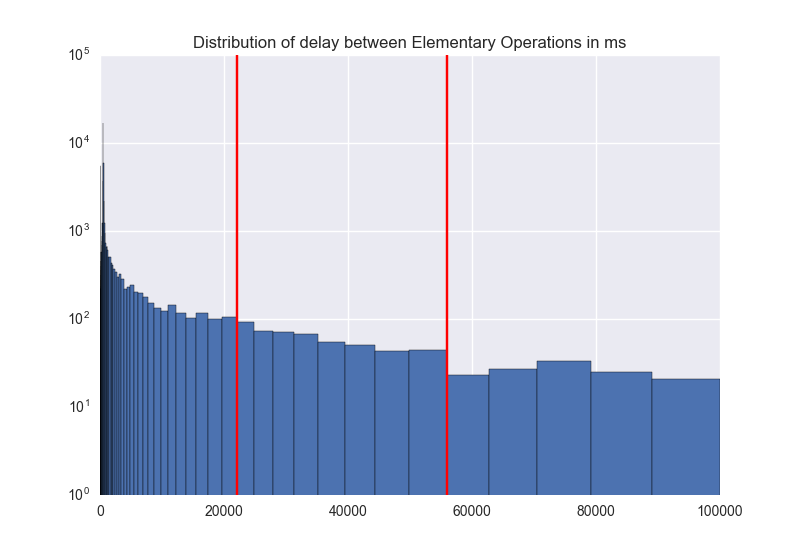
\includegraphics[scale=0.42]{figures/delay_between_elem_op.png}
\caption{Delay distribution between \texttt{ElementaryOperation} of the Belgian experiment}
\label{distribution_delay}
\end{figure}

We now focus on the classification of the \texttt{Operations} into a Write, Edit and Delete. The parameter that has to be tuned for this purpose is the number of characters that are added or deleted that differentiate a Write from an Edit and an Edit from a Delete, we call it \texttt{length\_edit}. We plot on Fig. \ref{len_edit} the distribution of the number of Write, Delete, Paste and Edit Operation with respect to the threshold number of characters to classify the \texttt{Operation} as an Edit. Again, there is no clear pattern and the number of Edit \texttt{Operations} increases logarithmically. We decided to select a length of 15 characters since the distribution stays constant from this point. The average number of characters in an English word is 5.1 \cite{Bochkarev} which supports our decision as it roughly means that deleting or adding less than three words is an Edit. Even though the Belgian experiment is not in English, it still provides a good intuition about what an Edit is.
\begin{figure}[h]
\centering
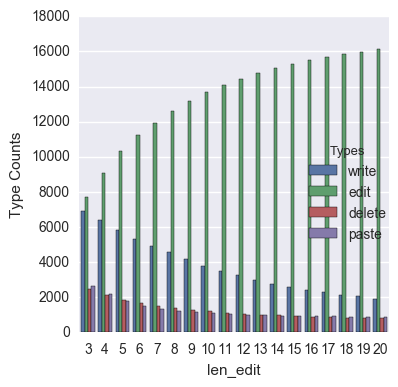
\includegraphics[scale=0.72]{figures/len_edit.png}
\label{len_edit}
\caption{\texttt{Operation} types distribution of the Belgian Experiment according to \texttt{length\_edit}}
\end{figure}

There are still three parameters to determine. Firstly, the maximum delay between two \texttt{Operations} to consider them as being synchronous. Then, the two timers to reset the Boolean for the short break on the one hand and the long break on the other hand. A common example for the short break is when the authors stop writing to drink coffee at the cafeteria. The long break has to be seen as at least spending one night without editing the \texttt{Pad}. These parameters depend on the task. Note that the long break metric is irrelevant for the Belgian Experiment as the \texttt{Pads} were edited for only 90 minutes. We set the delay for the long break to  8 hours which is supposed to be one night without editing the \texttt{Pad}. This means that it does not accurately show if it has taken several days to write the \texttt{Pad} but whether the \texttt{Pad} was written in one sitting or not. \\
We assume that on average a break lasts 22.8 minutes with a standard deviation of 25 minutes \cite{Daniel}, as we want to make sure not to miss breaks such as ‘social networking’ and to omit bathroom breaks. We arbitrarily lower bound the threshold for the short break delay to 10 minutes. \\
Finally for the synchronous delay that is the maximum time between two Operations from different authors to consider them synchronous, the proportion of synchronous edition increases linearly with the delay. We assume 3 minutes to be a reasonable guess.\\
Note that the selection of the parameters mentioned above is sometimes chosen relatively arbitrarily and these are determined based on the Belgian experiment which does not contain many documents. 

\subsection{Visualizations}
The text of the pad can be visualized as plain text, colored by Operation as shown on Fig.\ref{operations} or colored by authors.\\
In order to visualize the analytics we have been processing so far, we create the following plots. First we have the overall type distribution (without Jump) and the type distribution per user shown on Fig. \ref{types_per_user} (based on the text of Fig.\ref{operations}). 
\begin{figure}[h]
\centering
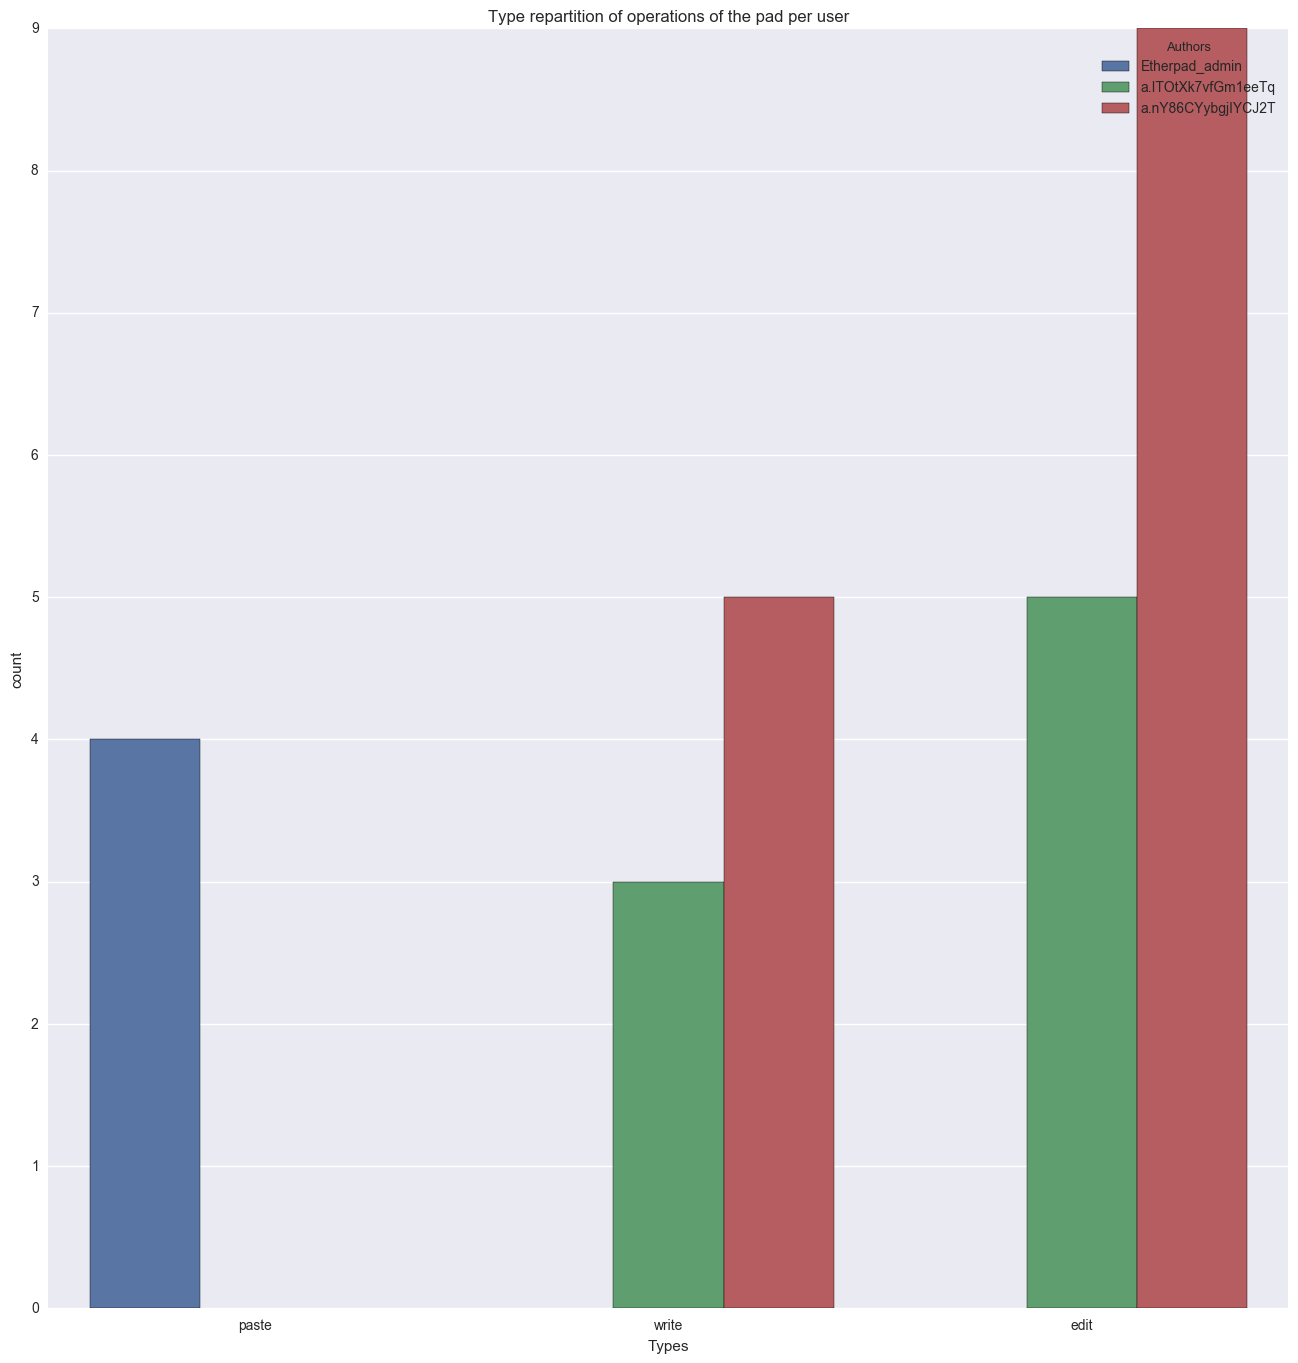
\includegraphics[scale=0.2]{figures/types_per_user.png}
\caption{Distribution \texttt{Operation} types per user}
\label{types_per_user}
\end{figure}
\\
We also plot the user participation proportion as a pie chart, the absolute user participation proportion per \texttt{Paragraph} and the user addition and deletion proportion per \texttt{Paragraph} shown on Fig. \ref{user_participation_para} (based on the same example).
\begin{figure}[h]
\centering
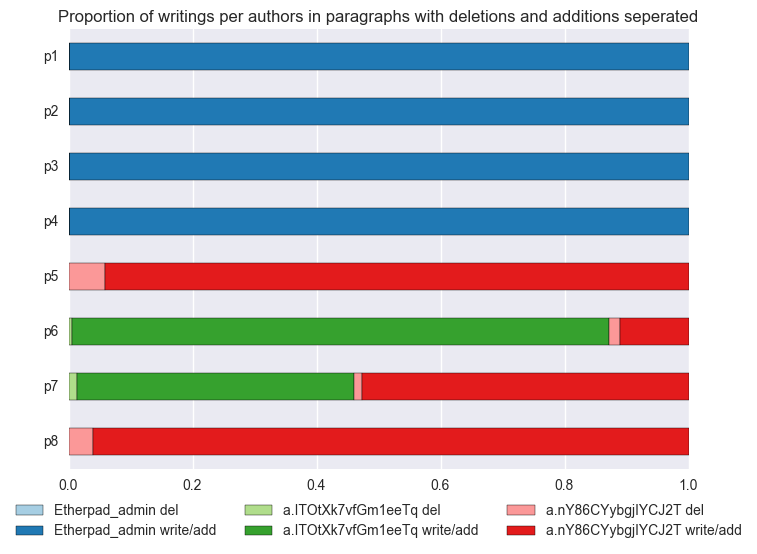
\includegraphics[scale=0.4]{figures/user_participation_para.png}
\caption{User participation proportion per \texttt{Paragraph}}
\label{user_participation_para}
\end{figure}
\\
Finally we plot the proportion of the \texttt{Pad} written synchronously shown on Fig. \ref{sync_prop_pad} and the proportion written synchronously per paragraph.
\begin{figure}[h]
\centering
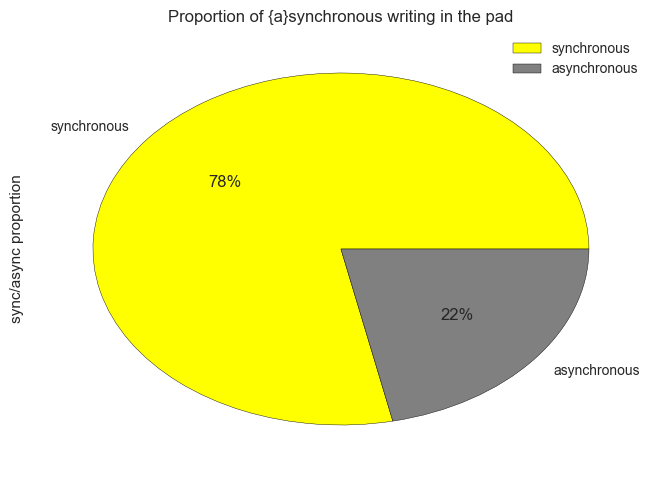
\includegraphics[scale=0.4]{figures/sync_prop_pad.png}
\caption{Proportion of \texttt{Pad} written synchronously}
\label{sync_prop_pad}
\end{figure}
\\
One can find all the detailed visualizations described above in our repository.
\\
\\
We now plot the evolution of the metrics described earlier. For this purpose, we use the Belgian experiment data and we keep only the last two hours of the pad‘s lifespan since they were created before being used. We split these pads into 32 periods and compute the scores for all periods for each 17 pads. We do not show here the evolution of all the metrics per pad for the sake of clarity. Some of the metrics are shown in Fig. \ref{boxplot_zoomed_Overall paste type score} for the overall paste score and in Fig. \ref{boxplot_zoomed_User proportion per paragraph score}.
\begin{figure}[h]
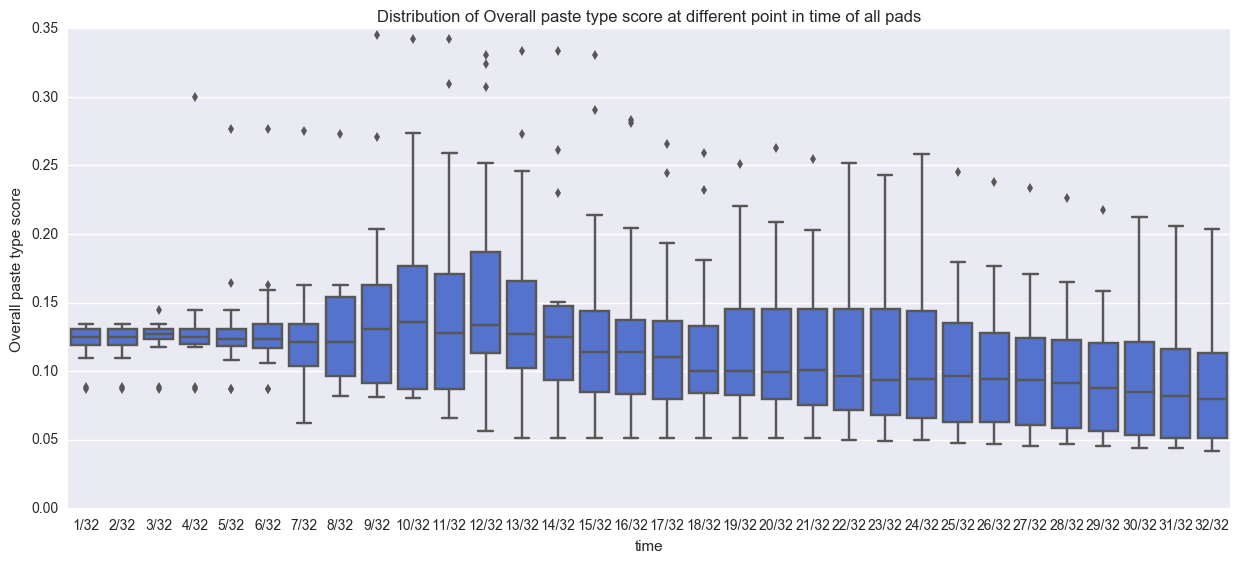
\includegraphics[scale=0.26]{figures/boxplot_zoomed_Overall_paste_type_score.png}
\caption{Evolution of the overall Paste score of the Belgian experiment}
\label{boxplot_zoomed_Overall paste type score}
\end{figure}

\begin{figure}[h]
\centering
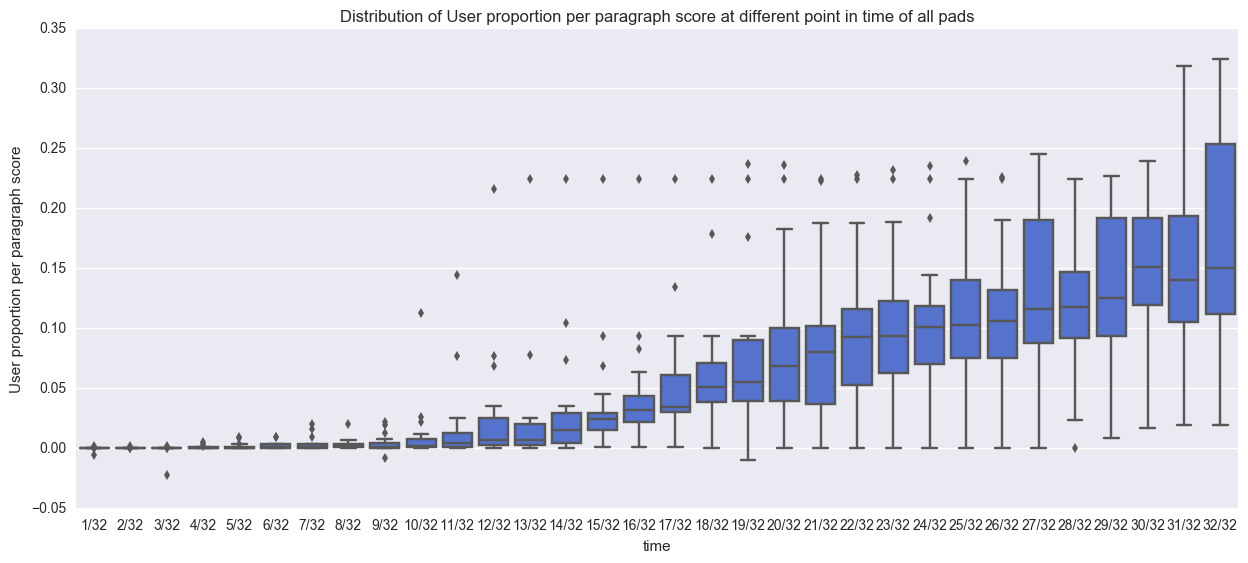
\includegraphics[scale=0.26]{figures/boxplot_zoomed_User_proportion_per_paragraph_score.png}
\caption{Evolution of the user proportion per \texttt{Paragraph}}
\label{boxplot_zoomed_User proportion per paragraph score}
\end{figure}

\subsection{Results Analysis}
In this section we will analyze the results that we obtain from the Belgian experiment. \\
Given the metrics evolution shown in the previous section, we can start making some observations. The overall paste score increases when students start editing the \texttt{Pad} and then it decreases until the end of the edition. Contrary to the edit, write and delete scores which increase . The user proportion per \texttt{Paragraph} score also increases as shown in Fig. \ref{boxplot_zoomed_User proportion per paragraph score}. This means that as the task is getting closer to the end, the students tend to copy and paste less but write, edit and delete more. Moreover, they participate more in each other’s paragraphs.\\
\\
We then look at the correlations between the metrics it is important  to note that all the correlations are close to zero-this means that all the metrics are highly uncorrelated and hence each one of them represents independent information. Our goal is to find different patterns in the writing manners. Thus  we try to cluster the \texttt{Pads}. To do so, we first apply KMeans with two clusters. Then, with  the resulting clustering, we apply a Principal Component Analysis in order to visualize our clustering and \texttt{Pads} on the two most important components and we show the results in Fig. \ref{PCA_kmeans}. With the exception of one outlier, we can see two clusters along the first component. This classification is mainly due to the User paste score which means that we can differentiate two groups of \texttt{Pad} by whether the Paste scores are  balanced or not amongst authors. This can simply be a coincidence and due to the low amount of data, we can not draw a meaningful conclusion yet, so we will not go further into this analysis of classification.
\begin{figure}[h]
\centering
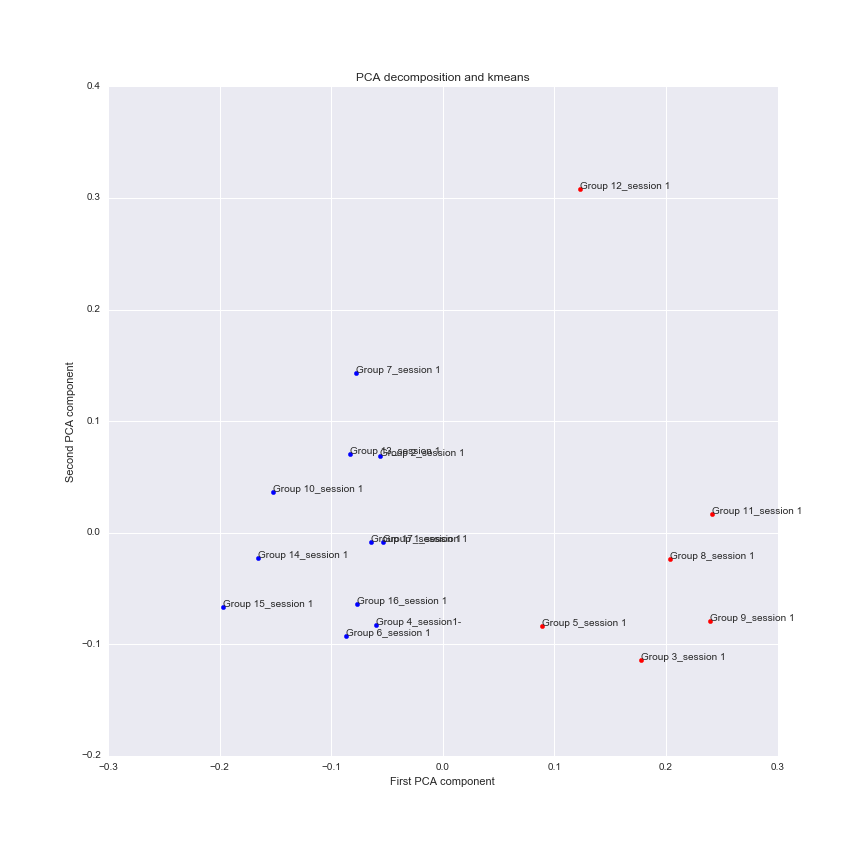
\includegraphics[scale=0.27]{figures/PCA_kmeans.png}
\caption{\texttt{Pads} represented in two clusters over the two principal components}
\label{PCA_kmeans}
\end{figure}
Finally, we make use of the pre-test questionnaire that the students had to answer after the task. The questions consist of various subjects related to personal and collaborative writings, such as planning, adjustments, communication, conflicts and revision. We compute correlations between the results of the form with the resulting metrics. The most highly correlated results are presented in Table \ref{table:corr}. Those results may be misleading due to the small amount of data we have and hence we cannot conclude any relation or make any prediction with certainty. Nevertheless, it is interesting to observe for example, that writers that do not find it useful to plan a text, usually take more short breaks. Also, authors that have a constructive win-lose approach, participate more in each other’s paragraphs. The full list of correlations can be found in our repository.

\begin{table}[h]
\begin{tabular}{|l|c|r|}
  \hline
  Pretest question & Metric & Corr. \\
  \hline
  My thoughts and ideas && \\
  become more clear to &&\\
  me as I write &&\\
  and rewrite & Sync score & 0.78 \\
  \hline
  Planning a text is not &Break&\\
  useful for me & score Short & 0.75 \\
  \hline
  When others disagree&&\\
  with me, I view it &&\\
  as an interesting&&\\
  opportunity to learn &&\\
  and to improve the &&\\
  quality of my ideas &&\\
  and reasoning. per &User& \\
  paragraph score& Proportion & 0.71 \\
  \hline
  Before I start to &&\\
  write, it is clear &&\\
  for me what I want &&\\
  to achieve with my &Alternating&\\
  readers & score & 0.68\\
  \hline
  When I disagree&& \\
  with others, I &&\\
  try to overpower &&\\
  them with my facts &Overall&\\
  and reasoning &Delete score & 0.67\\
  \hline
\end{tabular}
\caption{Highest correlations between metrics and pretest of the Belgian experiment}
\label{table:corr}
\end{table}


\section{Conclusion}

The results are not statically relevant because we only have access to 17 documents, but they look very promising. If we had to do a similar analysis with more \texttt{Pads}, we could find relations between collaboration or quality and our metrics with more statistical relevance. By enhancing this system with a bigger corpus, we could even aim at predicting the success of the collaboration in real time. For instance, if assignments and grades are given, one could use supervised machine learning in order to do a regression with our metrics-in order to predict the quality of the \texttt{Pad}. We could also combine our metrics into a single metric which would represent the overall collaboration score. This would give the teacher a quick insight on each group collaboration. \\
On a more technical side, it could be interesting to add a parsing for different writing events databases and even other editors. We also focus on the add/del operation, but it is important to also look at the format operations (changing to Bold/Italic/underlined…) as these could give us an additional insight on the collaboration between the authors. \\
Finally, it would also be valuable to explore the semantic of the text to better understand whether the users are collaborating (whether they are writing about the same topic, whether a user always writes about the same subject...).

\bibliographystyle{unsrt}
\bibliography{refs}

\end{document}
